\chapter{Procedure}
\section{The Cryostat}
\begin{figure}
	\centering
	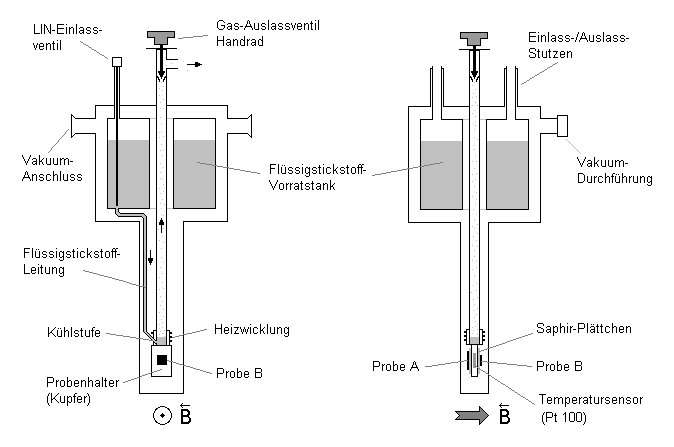
\includegraphics[width=.1\textwidth]{./img/cryostat.pdf}
	\captiond{The cryostat used in this experiment}{The sample chamber enclosed by a superconducting coil is visible in the center. Source: Lab manual}
\end{figure}
The cryostat used in this experiment is made up of a double-walled outer and inner glass dewar.
The inner dewar contains a sample chamber enclosed by a superconducting solenoid.
After evacuation of the inner dewar and its walls to clear out any residues, the walls are refilled with a small amount of helium and the inner dewar is flushed out with helium.
The outer dewar is filled with liquid nitrogen to cool down the samples (discussed in \autoref{sec:samples}).
At about \SIrange{80}{90}{\kelvin} liquid helium is poured into the inner dewar to speed up the cooling process.

\section{Resistance Over Temperature}
Resistances of the temperature sensor and all three samples are displayed on four digital bench multimeters.
To ensure simultaneous readout of all values, the multimeters are recorded with a video camera and the video is paused to read off a set of values.
From around \SI{60}{\kelvin}, temperatures are recorded with a carbon resistor instead of a platinum thermometer since it features a greater resolution for this temperature domain.
Resistances are measured for cooling down the samples as well as for warmup, where warming up the samples is accomplished by employing a PI-controlled heater to accurately sweep the temperature of the sample chamber.

\section{Critical Magnetic Field Over Temperature}
To plot the resistance of the Nb sample against the resistance of the temperature sensor, an $x$-$y$ plotter is used.
This $T$-$R$ curve is recorded for magnetic fields from \SIrange{0}{0.6}{\tesla} in \SI{0.1}{\tesla} increments to determine the dependence of the critical temperature on the magnetic field.
